\documentclass[11pt]{beamer}
\title{\textsc{Code2Inv}: A Deep Learning Framework for Program Verification}
\usepackage{verbatim}
\usepackage{amsmath}
\usepackage{amsthm}
\usepackage{graphics}
\usepackage{color}
\usepackage{stmaryrd}
\usepackage{multicol}

\newtheorem{proposition}{Proposition}

\date{\today}
\author{Xujie Si et al.}


\begin{document}
\maketitle

\begin{frame}\frametitle{Reference}
[1] Learning Loop Invariants for Program Verification.

[2] Code2Inv: Learning Loop Invariants for Program Verification.
\end{frame}

\begin{frame}\frametitle{Background}
\textbf{Counterexample-guided Inductive Synthesis(CEGIS):}

CEGIS is a classical paradigm for program verification where
\begin{itemize}
\item \textit{Generator} proposs a candidate solution.
\item \textit{Checker} determines whether the solution is correct or not. If not, provide counterexample to refine later.
\end{itemize}

\textbf{Shortcomes?}
\begin{itemize}
\item The framework does not utilize the info that can be directly taken from program source.
\item Candidate cannot be adaptive for the program.
\end{itemize}

\end{frame}

\begin{frame}\frametitle{Overview of \textsc{Code2Inv}}
\textsc{Code2Inv} is an extensible end-to-end  deep learing framework aims to compensate above shortcomes. The contribution of the tool is 
\begin{itemize}
\item A framework for program verification which leverage deep learning, reinforcement learning and attention mechanism..
\item Two small-scale instance of \textsc{Code2Inv}: loop invariant synthesizer and Constrained Horn Clause(CHC) Solver.
\end{itemize}
\end{frame}

\begin{frame}\frametitle{Idea of Invariant Synthesis}

The basic idea of this paper is to mimic how human experts reason the loop invariant.

\begin{example}
\begin{multicols}{2}
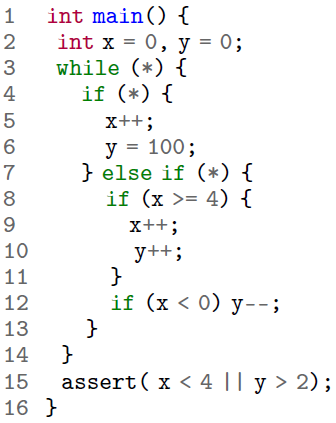
\includegraphics[scale = 0.45]{1.png}

\begin{itemize}
\item Start by reading the assertion. $x, y$.
\item $x$ may increase. $x < 4$ may not always hold.
\item How can $x \ge 4$: by executing the first branch $4$ times. Then we guess $y \ge 100$ because...
\item $x < 4 \vee y \ge 100$ is not enough, then add $x \ge 0$
\item $x \ge 0 \wedge (x < 4 \vee y \ge 100)$

\end{itemize}
\end{multicols}
\end{example}
\end{frame}

\begin{frame}\frametitle{Idea of Invariant Synthesis}

After going through the reasoning process three key components are concluded:
\begin{itemize}
\item Organize the program in a hierarchical structured way.
\item Compose the loop invariant step by step.

\item Focus on different part of the program at each step.
\end{itemize}

\end{frame}
\begin{frame}\frametitle{Preliminaries}
\begin{definition}[Multilayer Perceptron(MLP)]
A multilayer perceptron(MLP) is a basic neural network model approximating an arbitrary continuous function $\vec{y} =f^*(\vec{x})$, where $\vec{x}, \vec{y}$ are numeric vectors.
An MLP defines a mapping $\vec{y} = f(\vec{x};\theta)$.

\end{definition}

\begin{definition}[RNN]
An RNN approximate the mapping from a sequence of inputs $\vec{x}^1, \ldots, \vec{x}^t$ to either a single output $\vec{y}$ or a sequence of outputs $\vec{y}^1, \ldots, \vec{y}^t$. It defines a mapping $\vec{h}^t = f(\vec{h}^{t - 1}, \vec{x}^t; \theta)$.

A common RNN model are the long short-term memory network(LSTM) and gated recurrent units(GRUs).

\end{definition}

\textit{Remark.} GNN: commonly used to learn over graph structure data. It learns an embedding for each node of the given graph.
\end{frame}



\begin{frame}\frametitle{General Framework of \textsc{Code2Inv}}
\begin{multicols}{2}
\textbf{Domains of Program Structures:}
\begin{center}
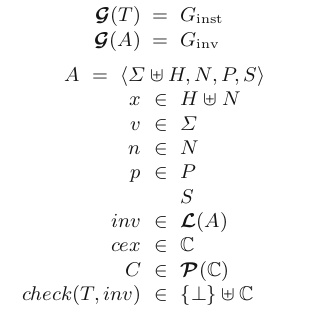
\includegraphics[scale=0.4]{programStruct.png}
\end{center}

\textbf{Domains of Neural Structures}
\begin{center}
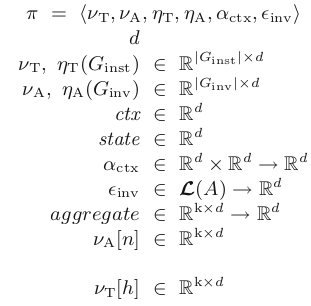
\includegraphics[scale=0.4]{NeuralPolicy.png}
\end{center}
\end{multicols}
\end{frame}

\begin{frame}\frametitle{General Framework of \textsc{Code2Inv}}
\begin{definition}[Neural Policy]
The neural policy is the key component of the framework and is define as 
\[\pi = \langle \nu_T, \nu_A, \eta_T, \eta_A, \alpha_{ctx}, \epsilon_{inv} \rangle \]

\end{definition}
Neural Policy is the most important component of the framework where 
\begin{itemize}
\item $\eta_T, \eta_A$ are two graph neural networks used for computing the neural embeddings  $\nu_T, \nu_A$ for graph representations  $G_{inst}, G_{inv}$ respectively.

\item $\alpha_{ctx}$ is a neural network implemented as GRU maintains the attention context $ctx$ when modifying invariant.

\item $\epsilon_{inv}$ implemented as a Tree-LSTM is an invariant encoder that encodes partial generated invariant into $state$, which is used to update the attention.
\end{itemize}



\end{frame}

\begin{frame}\frametitle{Overall Framework of Loop Invariant Synthesis}
\begin{center}
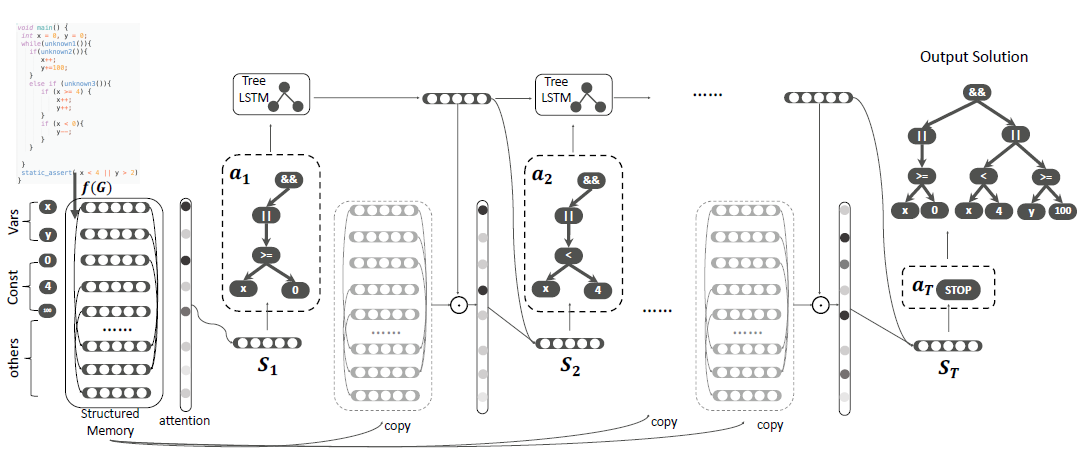
\includegraphics[scale = 0.39]{2.png}

\end{center}

\end{frame}


\begin{frame}\frametitle{General Framework of \textsc{Code2Inv}}
\begin{center}
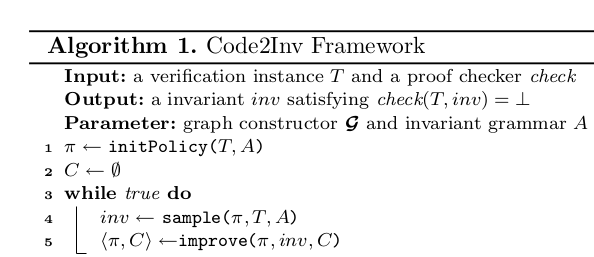
\includegraphics[scale=0.5]{algoMain.png}

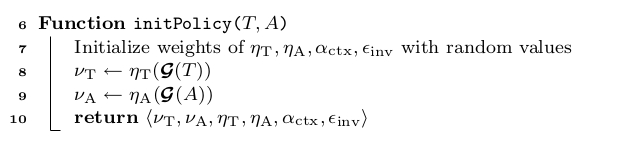
\includegraphics[scale=0.5]{algoInit.png}
\end{center}
\end{frame}

\begin{frame}\frametitle{Structured External Memory}
\begin{itemize}
\item First, convert a given program into a static single assignment form, then a flow graph where a vertex is an AST.

\item Then, convert the graph into vector representation. $E = \{(e_x^{(i)}, e_y^{(i)},e_t^{(i)})\}$.

\end{itemize}
\begin{center}

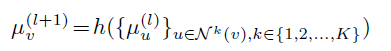
\includegraphics[scale = 0.4]{6.png}

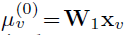
\includegraphics[scale = 0.4]{5.png}

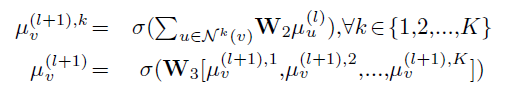
\includegraphics[scale = 0.4]{4.png}

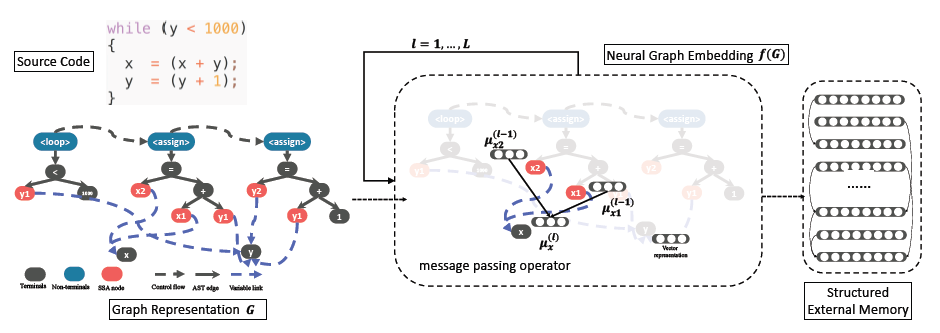
\includegraphics[scale = 0.4]{3.png}
\end{center}

\end{frame}

\begin{frame}\frametitle{General Framework of \textsc{Code2Inv}}
\begin{center}

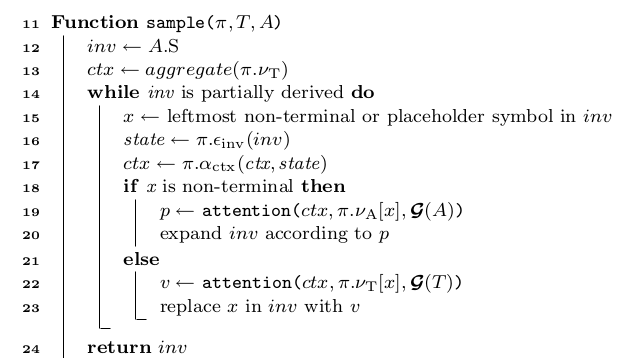
\includegraphics[scale=0.5]{algoSample.png}

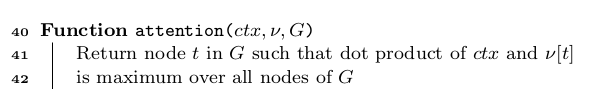
\includegraphics[scale=0.5]{algoAttention.png}
\end{center}
\end{frame}
\begin{frame}\frametitle{General Framework of \textsc{Code2Inv}}
\begin{center}

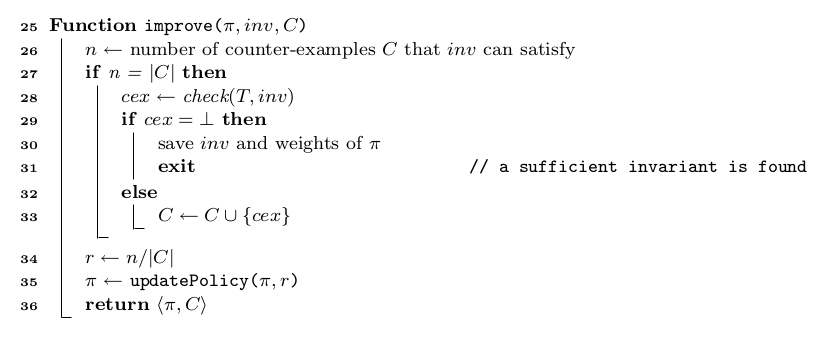
\includegraphics[scale=0.5]{algoImprove.png}

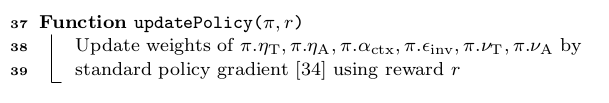
\includegraphics[scale=0.5]{algoUpdate.png}
\end{center}
\end{frame}




\begin{frame}\frametitle{Overall Framework of Loop Invariant Synthesis}
\begin{center}
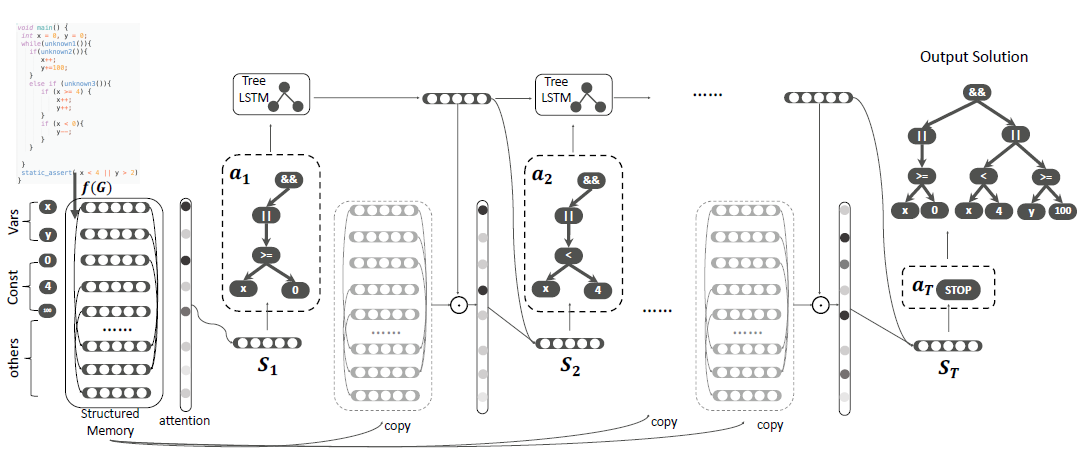
\includegraphics[scale = 0.39]{2.png}

\end{center}

\end{frame}
\begin{frame}\frametitle{Multi-Step Decision Making Process}
\begin{definition}[Loop Invariant]
We define the loop invariant to be a tree $\mathcal{T}$
\[\mathcal{T} = (\mathcal{T}_1 \vee \mathcal{T}_2\ldots) \wedge (\mathcal{T}_{t+1} \vee \mathcal{T}_{t+2}\ldots)\wedge \ldots \wedge (\ldots\mathcal{T}_{T - 1} \vee \mathcal{T}_{T})\]
\end{definition}

$T_t$ is $X < 2\times y + 10 - z$.

MDP: use MDP to model the problem of constructing the invariant incrementally.

$\mathcal{M}^G = (s_1, a_1, r_1, \ldots, s_T, a_T, r_T)$
\begin{itemize}
\item $a_t = (op_t, \mathcal{T}_t)$. $op_t$ can be $\wedge $ or $\vee $.
\item $s_t = (G, \mathcal{T}^{ < t})$.

\end{itemize}

\end{frame}

\begin{frame}\frametitle{Reward Design $r_t$}
\textbf{Early Reward}: the goal is to quickly remove the trivial and meaningless predicates. e.g. $e == e, e < e$. Examine partially generated $\mathcal{T}^t$.


\begin{center}
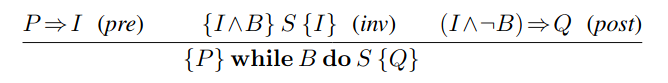
\includegraphics[scale=0.4]{inv.png}
\end{center}
\textbf{Continuous Reward}: $ce_{pre}, ce_{inv}, ce_{post}$ and $pass_{pre}, pass_{inv}, pass_{post}$.
No new counterexample is introduced: 
\begin{center}
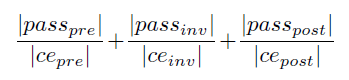
\includegraphics[scale = 0.5]{7.png}
\end{center}
New counterexample introduced: 
\begin{center}
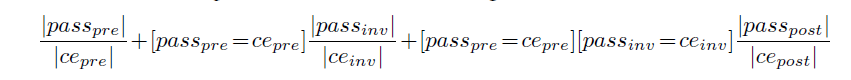
\includegraphics[scale=0.5]{8.png}

\end{center}
\end{frame}


\begin{frame}\frametitle{Termination}
Situations for termination:
\begin{itemize}
\item Successfully generated.
\item The tree of the generated invariant reach a ceiling number of branches.
\item The agent generate invalid action.

\end{itemize}

\end{frame}
\begin{frame}\frametitle{Experimental Result}

\begin{center}

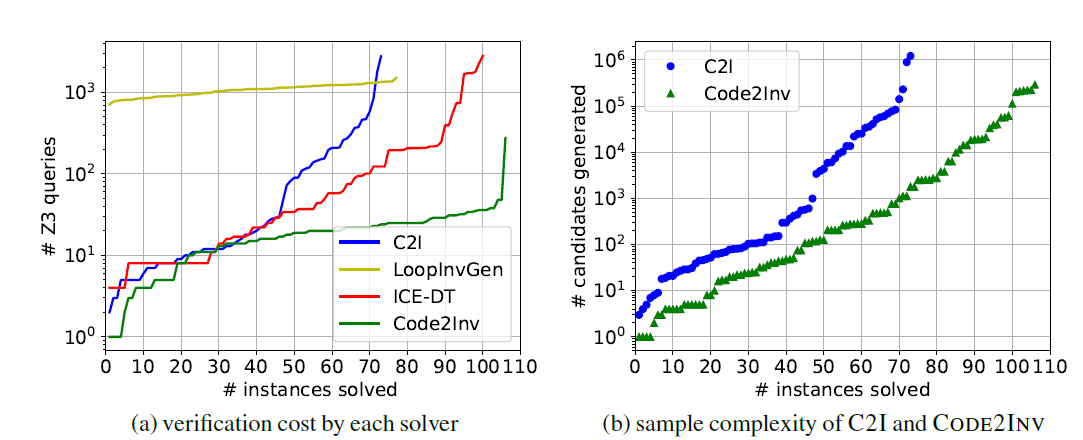
\includegraphics[scale = 0.35]{10.png}
\end{center}

\end{frame}

\begin{frame}\frametitle{Ablation Study}
\begin{center}
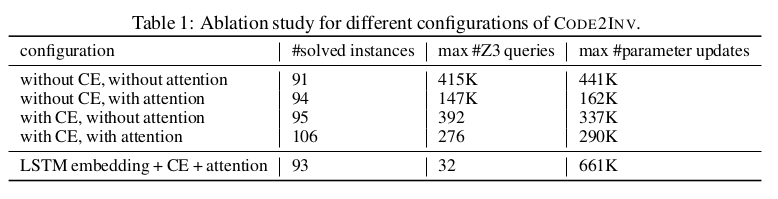
\includegraphics[scale=0.4

]{ablation.png}
\end{center}
\end{frame}
\end{document}